\documentclass[practic, labs]{BMSTU-IU7}
\usepackage{biblatex}
\usepackage{listings}
\usepackage{csvsimple}

\usepackage{caption}
\usepackage{algorithm2e}

\usepackage{geometry}
\geometry{verbose,a4paper,bmargin=2cm}

\lstset{
	language=Python,
	numbers=left,
	captionpos=t,
	frame=single,  % Отображение рамки вокруг кода
	backgroundcolor=\color{white}
}

\bibliography{biblio}

\student{Дьяченко А. А.}
\group{ИУ7-53Б}
\labsNumber{5}
\theme{<<Организация асинхронного взаимодействия потоков вычисления на примере конвейерных вычислений>>}
\speciality{<<Анализ алгоритмов>>}
\supervisor{Строганов Д. В.}

\addbibresource{biblio.bib}


\begin{document}
	\maketitle
	
	\setcounter{page}{3}
\renewcommand{\contentsname}{Содержание}
\tableofcontents
	\section*{ВВЕДЕНИЕ}
\addcontentsline{toc}{section}{ВВЕДЕНИЕ}

<<<<<<< HEAD:passed/lab_01/report/src/02-intro.tex
Целью данной лабораторной работы является изучение расстояния Левенштейна и Дамерау~---~Левенштейна.

Расстояние Левенштейна (редакционное расстояние) и его модификация - расстояние Дамерау~---~Левенштейна, представляют собой метрики, используемые для измерения различий между двумя последовательностями символов.
=======
Целью данной лабораторной работы является изучение расстояния Левенштейна и Дамерау--Левенштейна.

Расстояние Левенштейна (редакционное расстояние) и его модификация - расстояние Дамерау--Левенштейна, представляют собой метрики, используемые для измерения различий между двумя последовательностями символов.
>>>>>>> 786b864 (lab_01 almost passed):lab_01/report/src/02-intro.tex
Они определяют минимальное количество односимвольных операций (вставка, удаление, замена и транспозиция), необходимых для преобразования одной последовательности символов в другую.
Эти метрики были разработаны советским математиком Владимиром Левенштейном в 1965 году и модифицированы впоследствии с учетом операции транспозиции символов, получив название расстояния Дамерау--Левенштейна.

Расстояние Левенштейна и его модификация имеют широкий спектр применений в различных областях, включая компьютерную лингвистику (автозамена, исправление ошибок), биоинформатику (анализ генома, белковых последовательностей).

Задачи лабораторной работы:
\begin{itemize}
    \item реализация алгоритмов с использованием динамического программирования;
    \item сравнение требуемого времени выполнения в тактах процессора и занимаемой памяти;
    \item подготовка отчёта по лабораторной работе.
\end{itemize}


	\section{Аналитическая часть}

<<<<<<< HEAD
Классический (стандартный) алгоритм перемножения матриц --- реализация математического определения умножения матриц.
=======
<<<<<<< HEAD
<<<<<<< HEAD
Классический (стандартный) алгоритм перемножения матриц --- реализация математического определения умножения матриц.
=======
Классический (стандартный) алгоритм перемножения матриц - реализация математического определения умножения матриц.
>>>>>>> 7ad89dc (lab_02 almost passed)
=======
Классический (стандартный) алгоритм перемножения матриц --- реализация математического определения умножения матриц.
>>>>>>> af69c2c (lab_02 passed)
>>>>>>> fb5d8bb (lab_02 passed)
Имеет ассимптотическую сложность \(O(n^{3})\).

Алгоритм Винограда имеет ассимптотическую сложность \(O(n^{2.3755})\), поэтому является одним из самых эффективных по времени алгоритмом умножения матриц \cite{Виноград}. 

Алгоритм Штрассена имеет ассимптотическую сложность \(O(n^{2.78})\) \cite{Ultra-Fast}. 
Идея этого метода состоит в открытии того, что произведение С двух матриц А и В размером 2×2 можно вычислить с помощью только семи, а не восьми умножений, которые необходимы при использовании стандартного алгоритма \cite{Штрассен}.
	\section{Конструкторская часть}

В этом разделе будут представлены схемы реализуемых алгоритмов.

\subsection{Полный перебор}

На рисунке~\ref{fig:bruteforce} приведена схема алгоритма решения задачи коммивояжера полным перебором. 

\begin{figure}
	\centering
	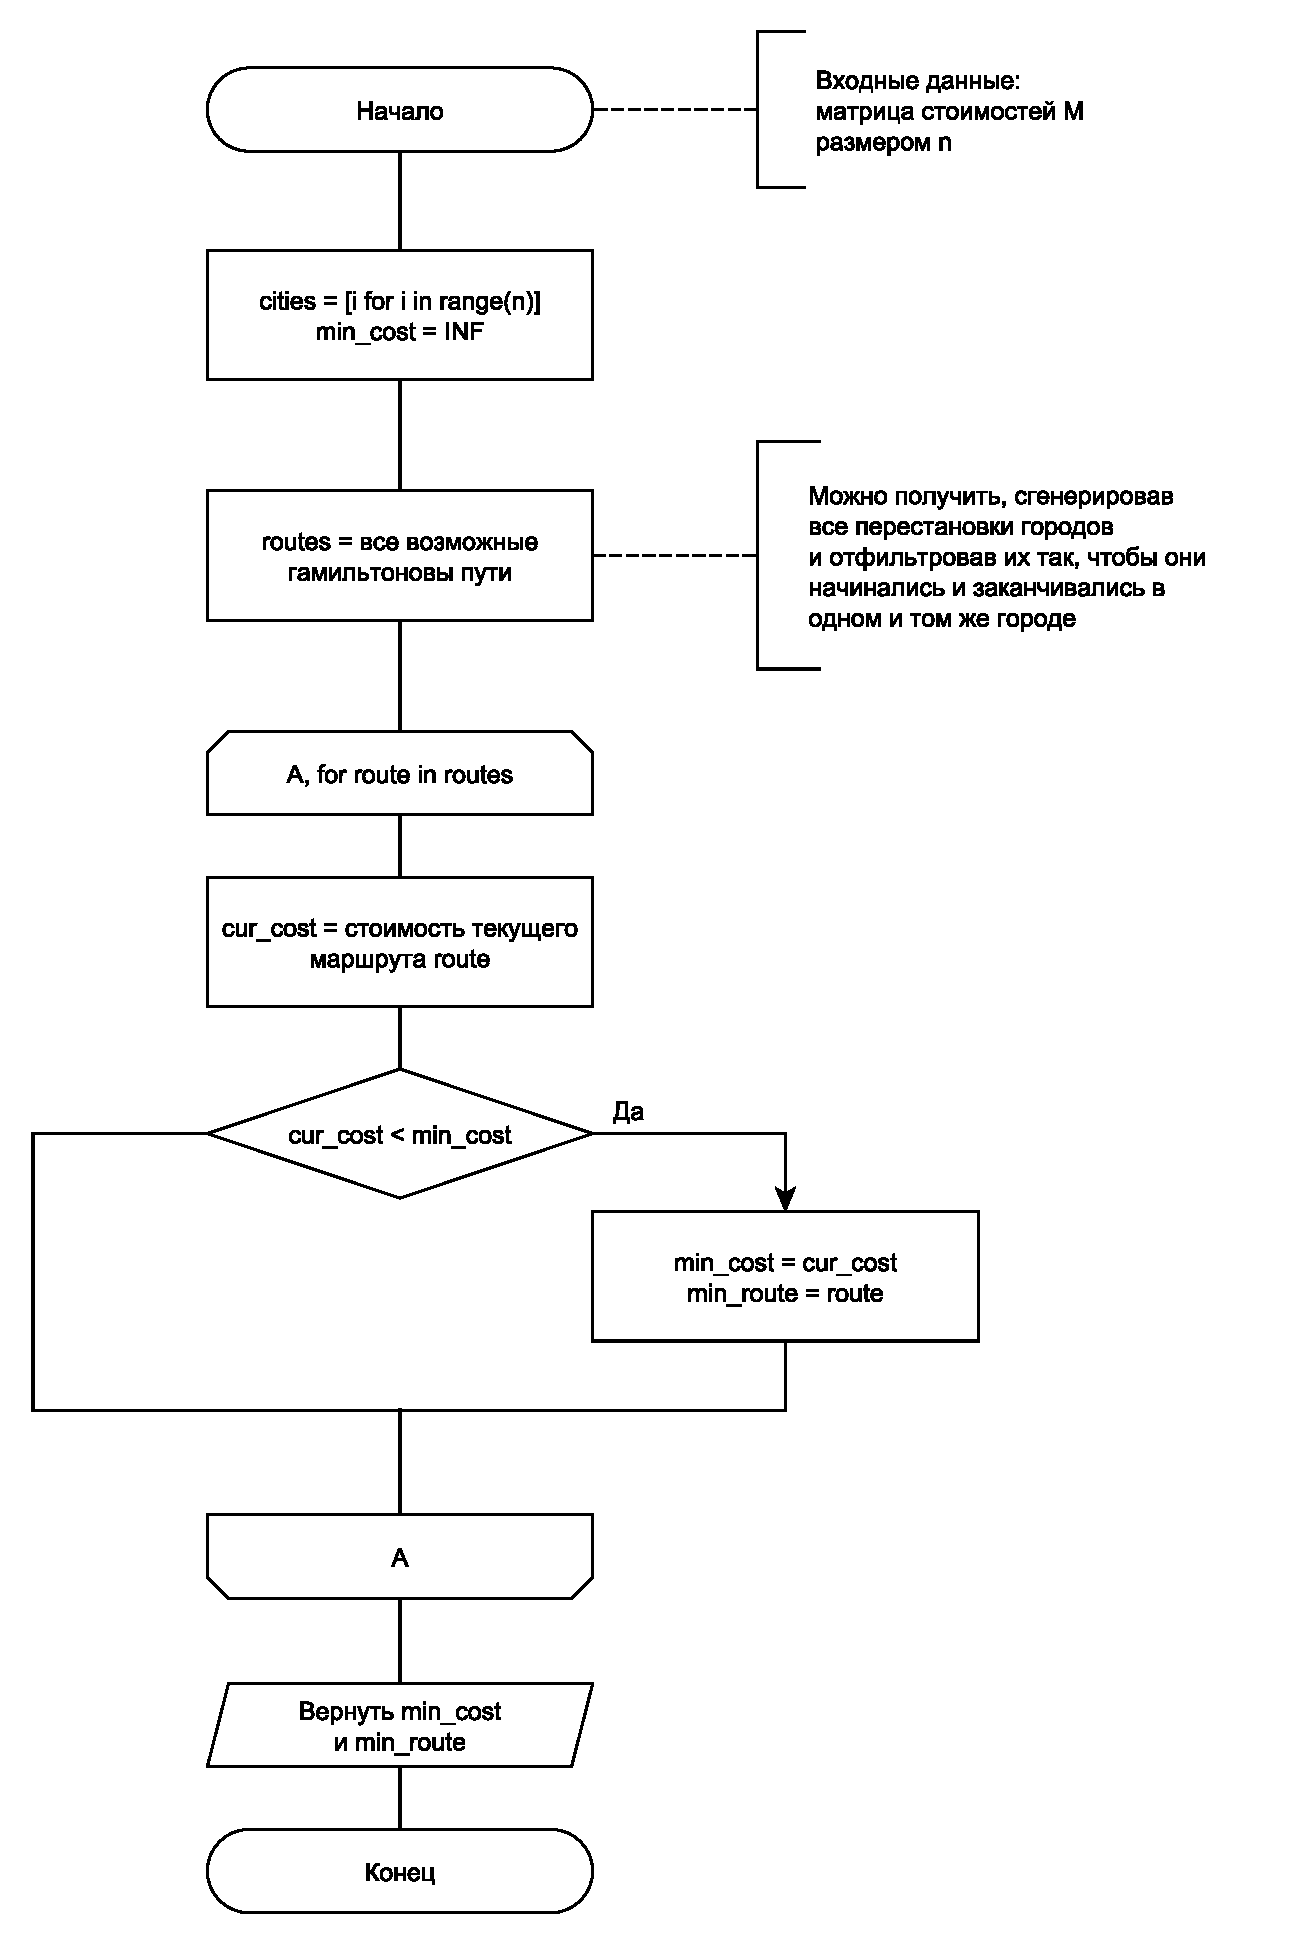
\includegraphics[width=0.65\linewidth]{images/bruteforce}
	\caption{Полный перебор}
	\label{fig:bruteforce}
\end{figure}

Преимущество алгоритма: оптимальный путь будет найден всегда.

Недостаток: скорость.

\subsection{Муравьиный алогритм}

На рисунке~\ref{fig:ant} приведена схема алгоритма решения задачи коммивояжера муравьиным алгоритмом. 

\begin{figure}
	\centering
	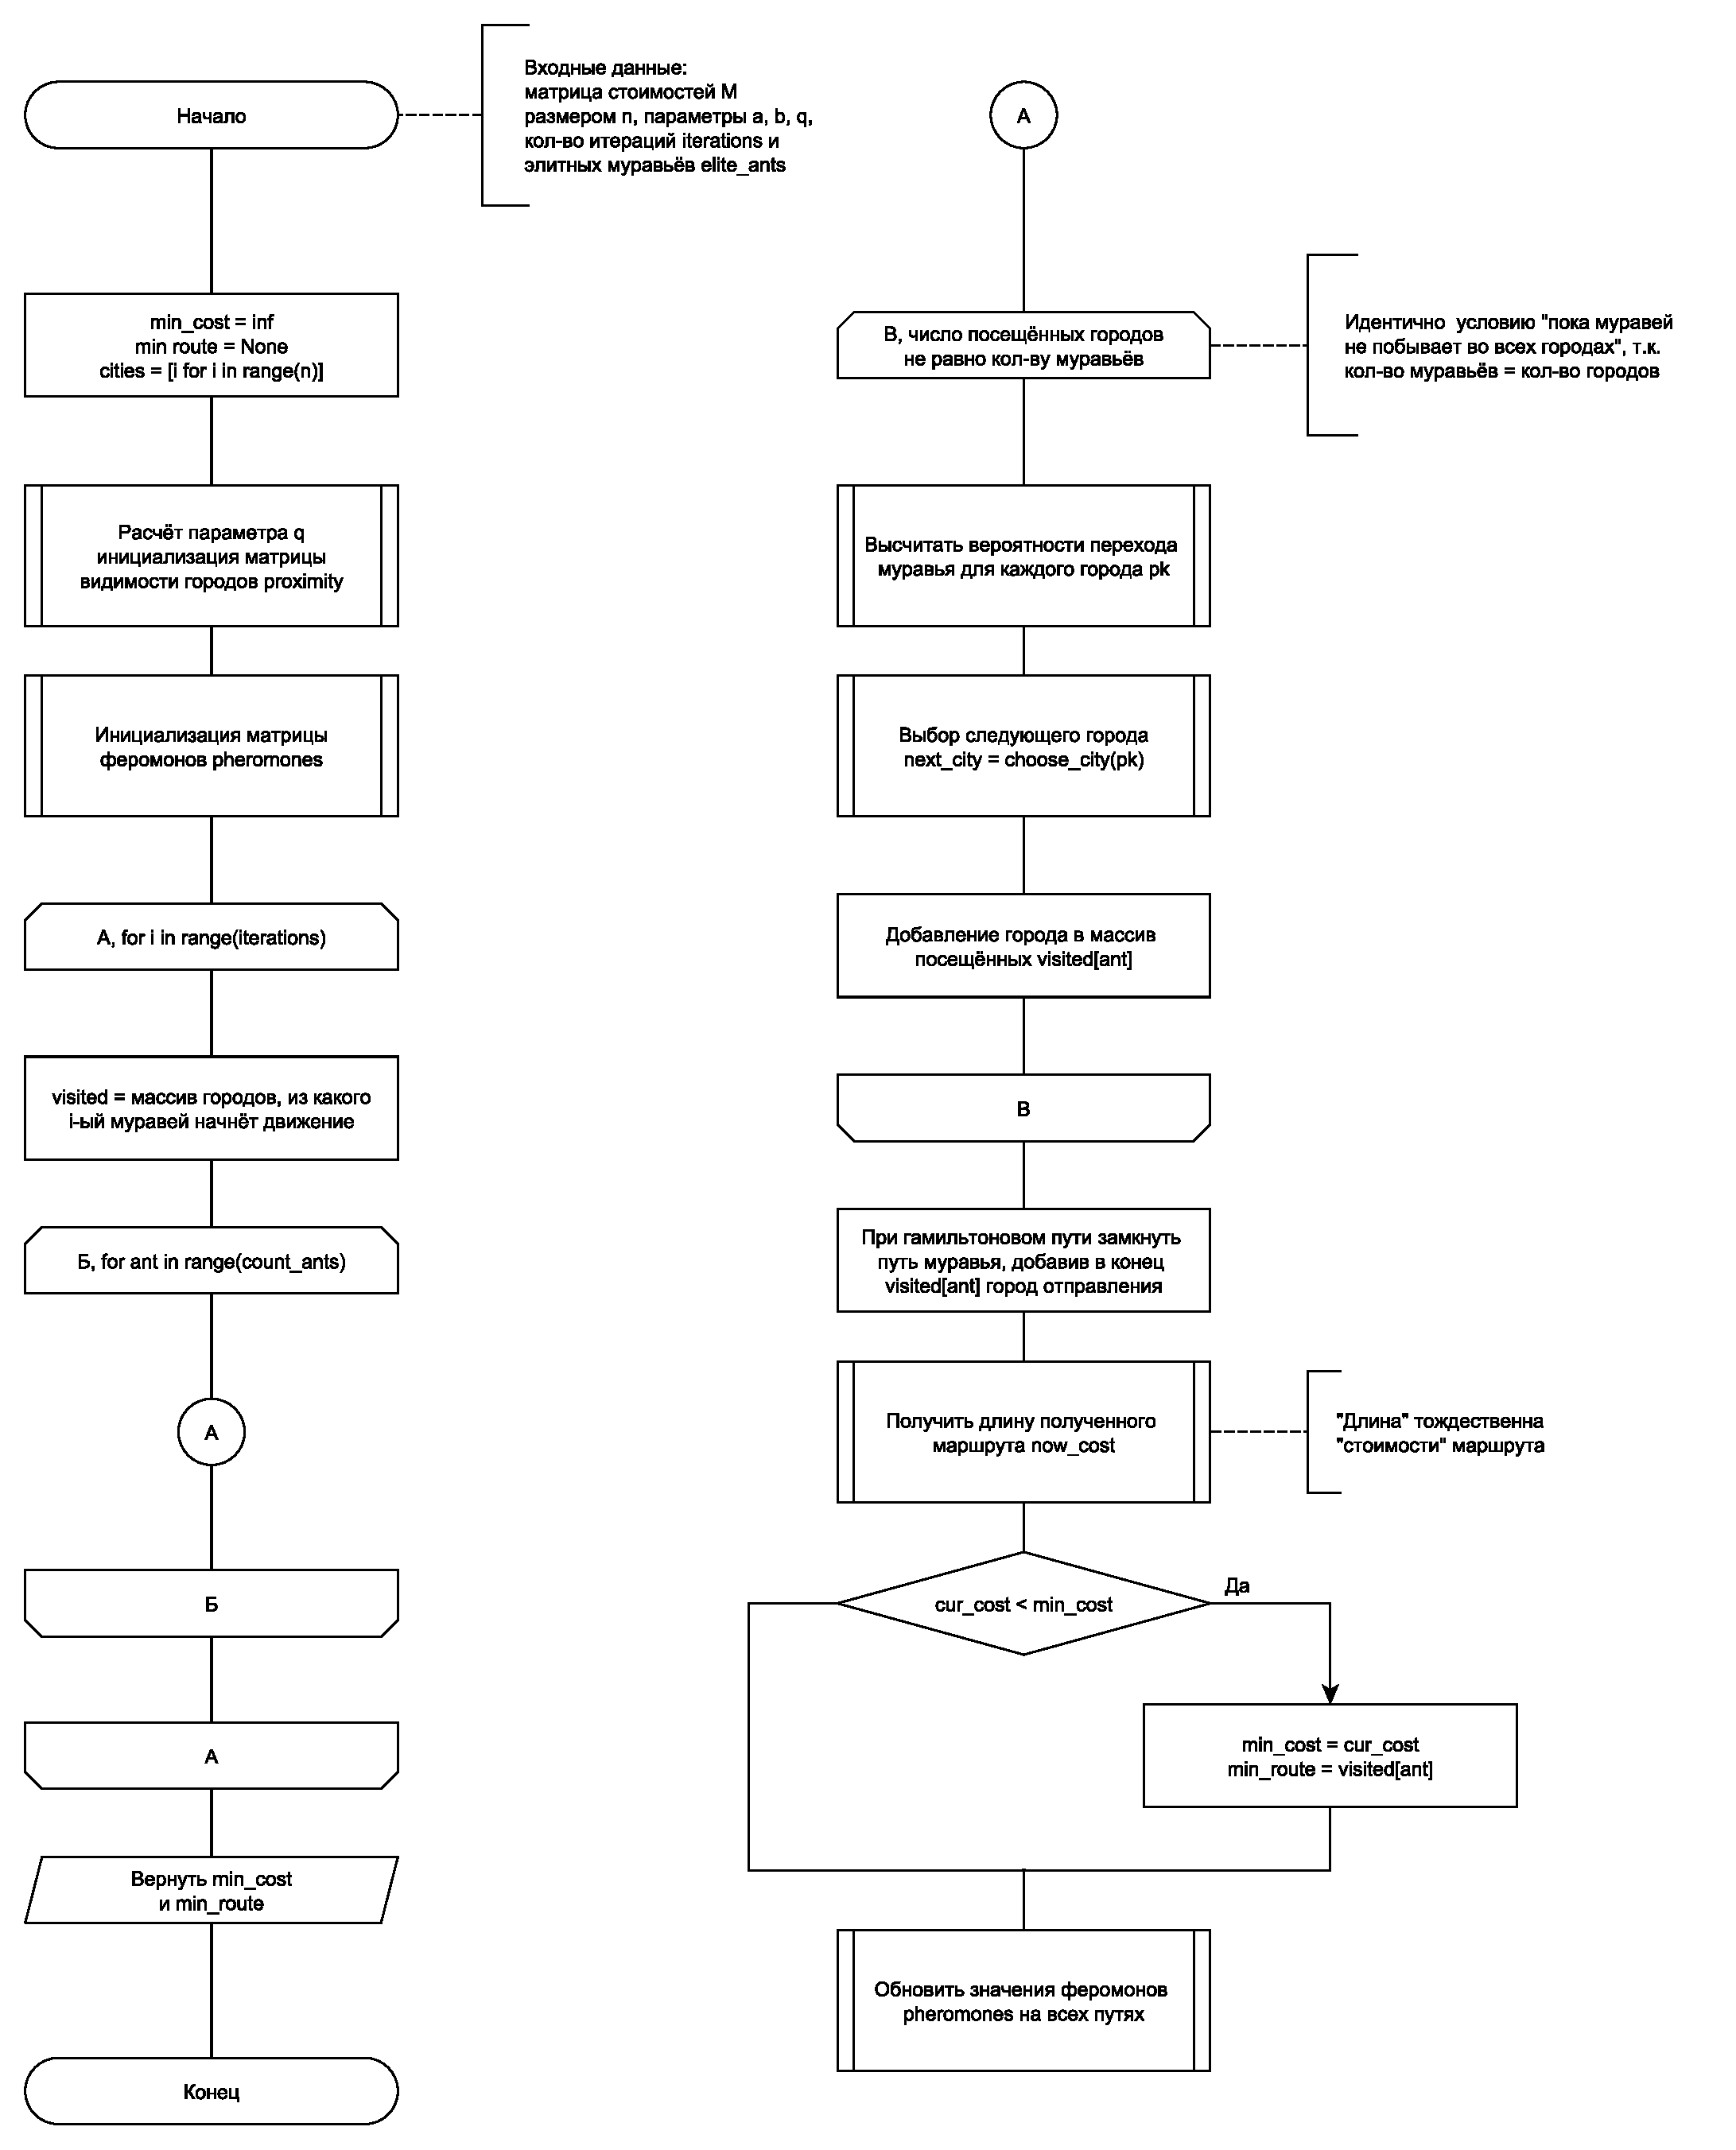
\includegraphics[width=1.0\linewidth]{images/ant}
	\caption{Муравьиный алгоритм}
	\label{fig:ant}
\end{figure}

На рисунке~\ref{fig:probabilities} приведена схема алгоритма вычисления вероятностных переходов.

\begin{figure}
	\centering
	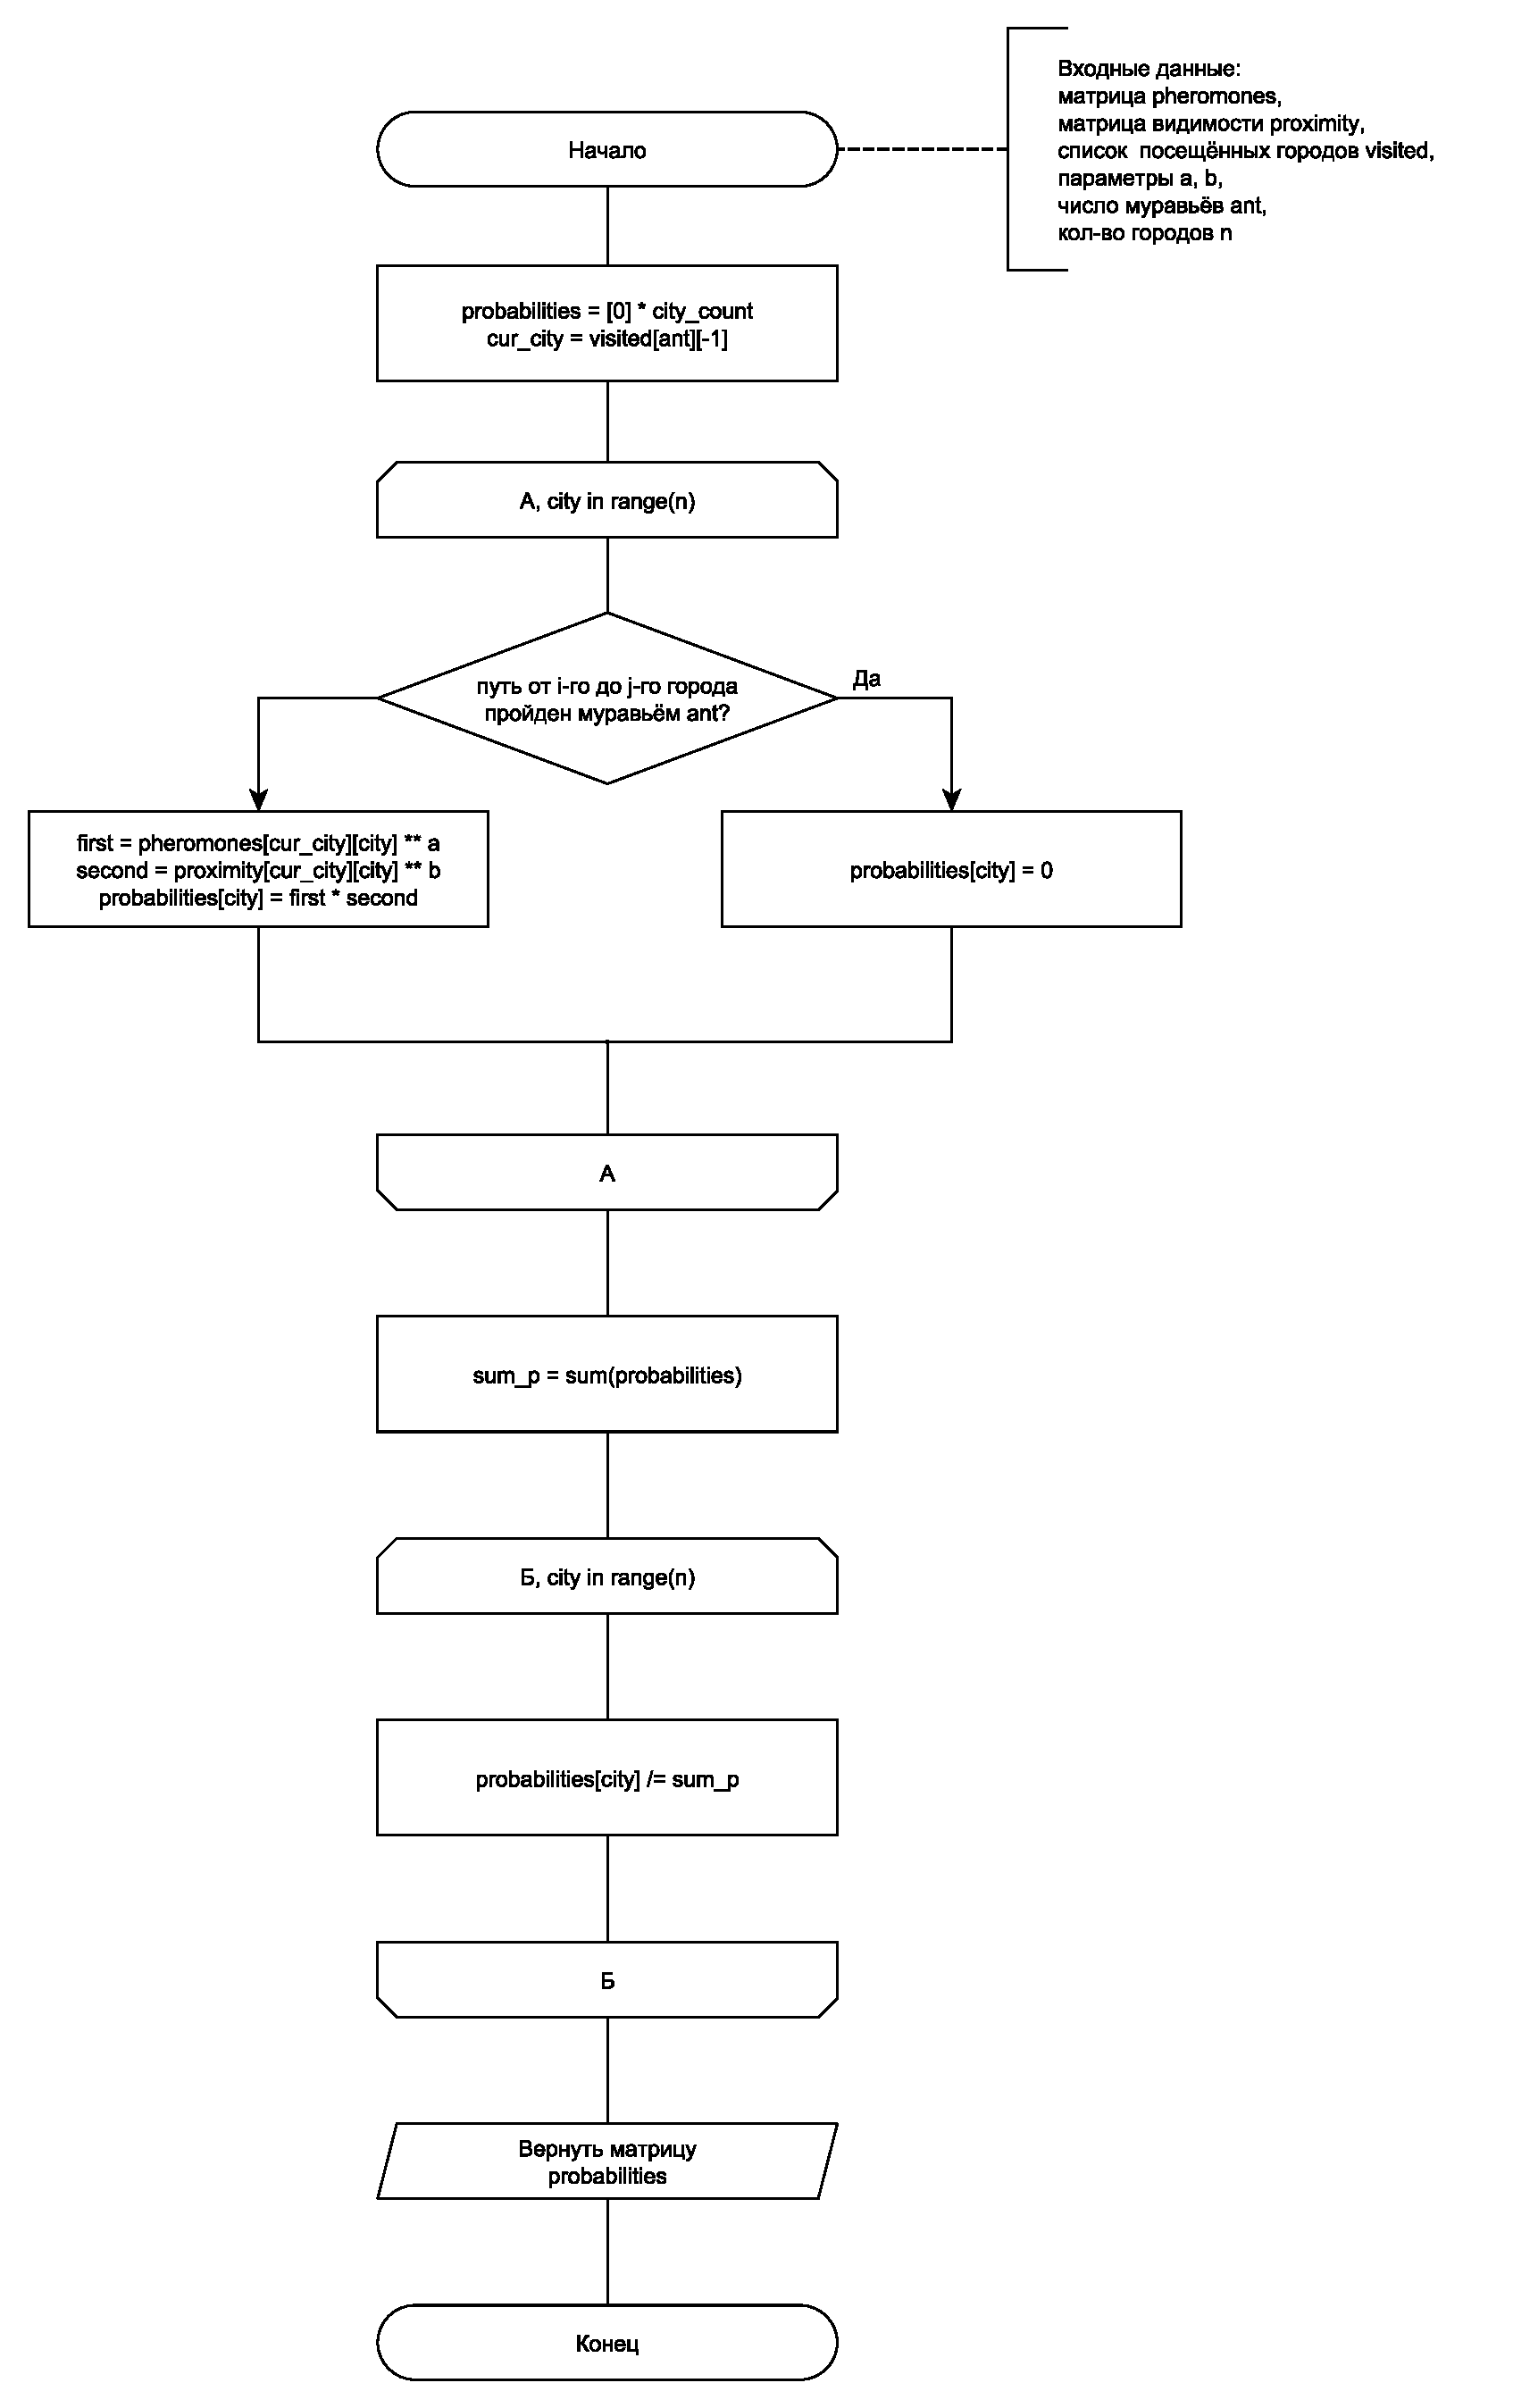
\includegraphics[width=0.85\linewidth]{images/probabilities}
	\caption{Вычисление вероятностных переходов}
	\label{fig:probabilities}
\end{figure}

На рисунке~\ref{fig:pheromone} приведена схема алгоритма обновления кол-ва феромонов на путях.

\begin{figure}
	\centering
	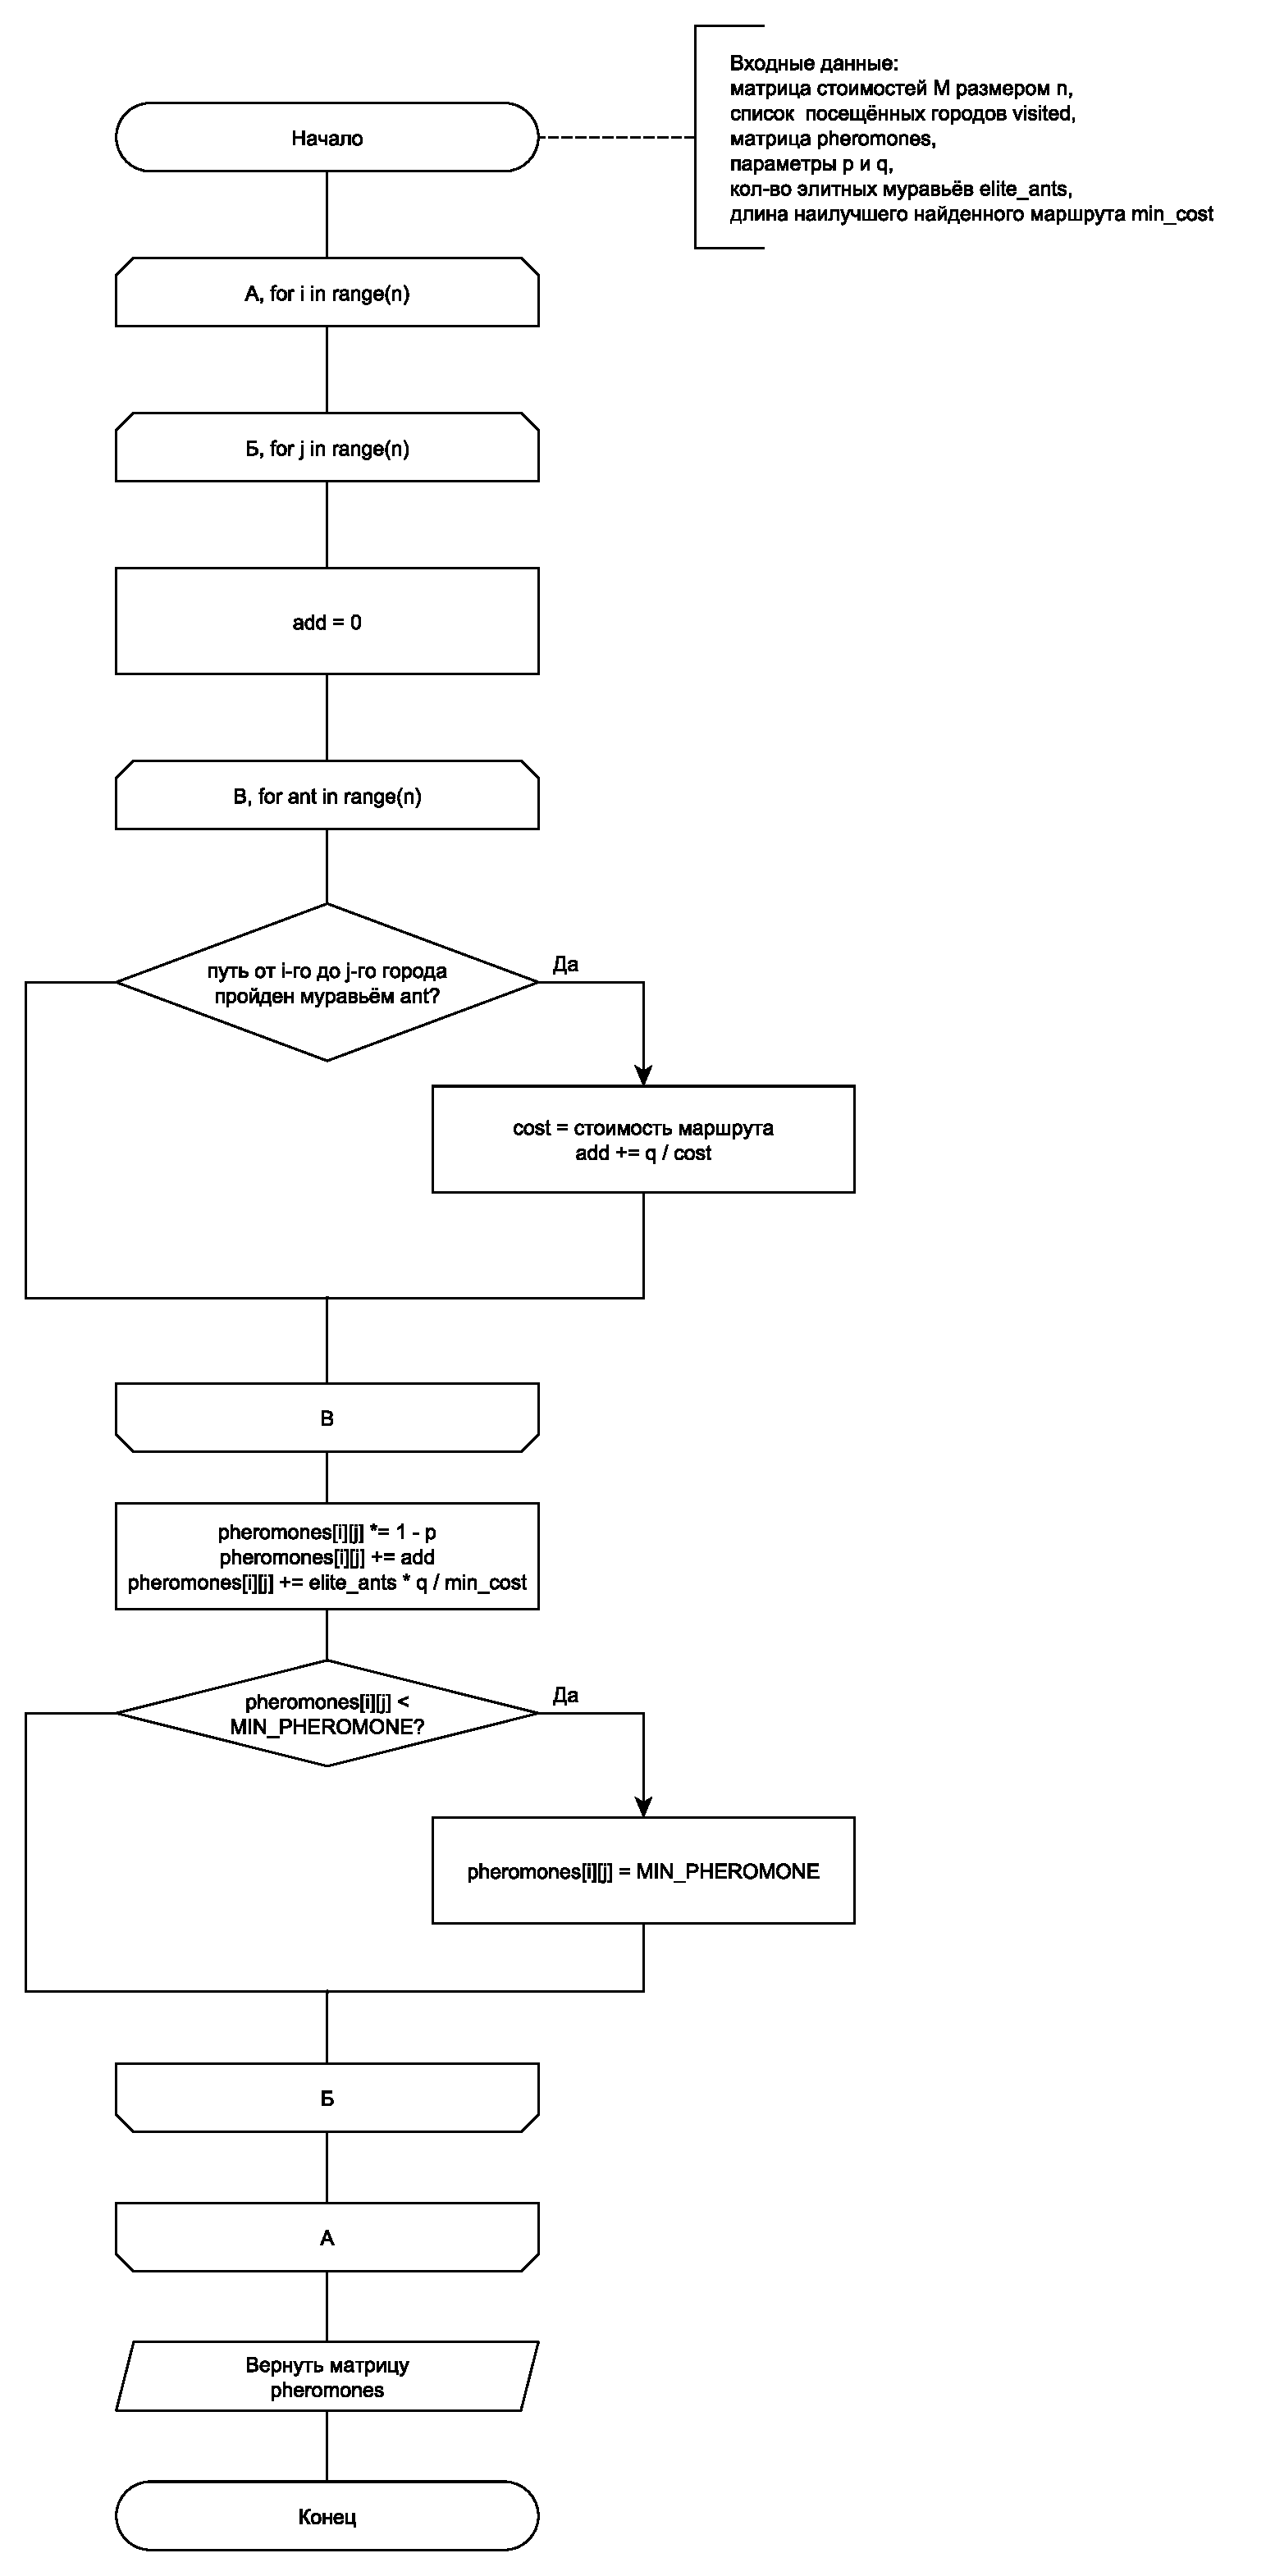
\includegraphics[width=0.65\linewidth]{images/pheromone}
	\caption{Обновление феромона}
	\label{fig:pheromone}
\end{figure}

Обратите внимание: по варианту необходимо рассмотреть муравьиный алгоритм с элитными особями.
Элитный муравей усиливает ребра наилучшего маршрута, найденного с начала работы алгоритма \cite{штовба2003муравьиные}.
Именно поэтому к значению $pheromones[i][j]$ добавляется значение $\dfrac{elite\_ants \cdot q}{ min\_cost}$.
В алгоритме без элитных муравьёв этого слагаемого нет.

Остальные схемы подпрограмм, указанные на рисунке~\ref{fig:ant} не приведены, т.к. они зависят от конкретной реализации.
Подпрограммы рисунках~\ref{fig:probabilities} и~\ref{fig:pheromone}, в свою очередь, от реализации к реализации не меняются (за исключением модификаций метода, таких как добавление элитных муравьёв).

Преимущество метода: скорость.

Недостаток: для нахождения оптимального пути требуется увеличение итераций и подбор параметров опытным путём.
	\section{Технологическая часть}
В данном разделе приведены требования к программному обеспечению, средства реализации и листинги кода.

\subsection{Требования к ПО}

К программе предъявляется ряд требований:
\begin{itemize}
	\item на вход подаются две строки на русском или английском языке в любом регистре;
	\item на выходе -- искомое расстояние для трёх методов и их время выполнения.
\end{itemize}

\subsection{Средства реализации}

В качестве языка программирования для реализации лабораторной работы был выбран С++.

Данный выбор обусловлен поддержкой языком парадигмы объектно -- ориентированного программирования и наличием библиотек для точного замера времени.

Время выполнения реализации алгоритмов было замерено с помощью библиотеки \textit{chrono}.

\subsection{Сведения о модулях программы}
Программа состоит из трех программных модулей:
\begin{enumerate}[label={\arabic*)}]
	\item main.cpp -- главный модуль программы, содержащий функцию main и замер времени;
	\item algorithm.cpp, algorithm.h -- модуль с реализацией алгоритмов;
	\item menu.cpp, menu.h -- модуль с выбором режима работы программы;
	\item tests.cpp, tests.h -- модуль с тестированием программы.
\end{enumerate}

\newpage
\subsection{Реализация алгоритмов}

В листингe \ref{lst:algo1} приведена реализация итеративного алгоритма нахождения расстояния Левенштейна.


\begin{lstinputlisting}[
	label={lst:algo1},
	caption={Итеративный алгоритм нахождения расстояния Левенштейна},
	]{listings/lev.cpp}
\end{lstinputlisting}

\newpage
В листингe \ref{lst:algo2} приведена реализация итеративного алгоритма нахождения расстояния Дамерау--Левенштейна.

\begin{lstinputlisting}[
<<<<<<< HEAD
<<<<<<< HEAD:passed/lab_01/report/src/05-techn.tex
	caption={Итеративный алгоритм нахождения расстояния Дамерау~---~Левенштейна},
=======
	caption={Итеративный алгоритм нахождения расстояния Дамерау--Левенштейна},
>>>>>>> 786b864 (lab_01 almost passed):lab_01/report/src/05-techn.tex
=======
	caption={Итеративный алгоритм нахождения расстояния Дамерау~---~Левенштейна},
>>>>>>> f0c1fd9 (lab_01 passed)
	label={lst:algo2}
	]{listings/dlev.cpp}
\end{lstinputlisting}

\newpage
В листингe \ref{lst:algo3} приведена реализация рекурсивного алгоритма нахождения расстояния Дамерау--Левенштейна.

\begin{lstinputlisting}[
<<<<<<< HEAD
<<<<<<< HEAD:passed/lab_01/report/src/05-techn.tex
	caption={Рекурсивный алгоритм нахождения расстояния Дамерау~---~Левенштейна},
=======
	caption={Рекурсивный алгоритм нахождения расстояния Дамерау--Левенштейна},
>>>>>>> 786b864 (lab_01 almost passed):lab_01/report/src/05-techn.tex
=======
	caption={Рекурсивный алгоритм нахождения расстояния Дамерау~---~Левенштейна},
>>>>>>> f0c1fd9 (lab_01 passed)
	label={lst:algo3}
	]{listings/dlev_req.cpp}
\end{lstinputlisting}

\newpage
В листингe \ref{lst:algo4} приведена реализация рекурсивного алгоритма нахождения расстояния Дамерау--Левенштейна с кэшем.

\begin{lstinputlisting}[
<<<<<<< HEAD
<<<<<<< HEAD:passed/lab_01/report/src/05-techn.tex
	caption={Рекурсивный алгоритм нахождения расстояния Дамерау~---~Левенштейна с кэшем},
=======
	caption={Рекурсивный алгоритм нахождения расстояния Дамерау--Левенштейна с кэшем},
>>>>>>> 786b864 (lab_01 almost passed):lab_01/report/src/05-techn.tex
=======
	caption={Рекурсивный алгоритм нахождения расстояния Дамерау~---~Левенштейна с кэшем},
>>>>>>> f0c1fd9 (lab_01 passed)
	label={lst:algo4}
	]{listings/dlev_req_cache.cpp}
\end{lstinputlisting}
	\section{Исследовательская часть}

\subsection{Технические характеристики}

Технические характеристики устройства, на котором выполнялся замерный эксперимент:
\begin{itemize}[label*=---]
	\item операционная система Windows 11;
	\item память 16 ГБ;
	\item процессор 3,6 ГГц 6-ядерный процессор AMD Ryzen 5000 series 5.
\end{itemize}

Замеры проводились на ноутбуке, включенном в сеть электропитания. 
Во время тестирования ноутбук был нагружен только интегрированной средой разработки и непосредственно выполняемой программой.

\subsection{Пример работы программы}

На рисунке \ref{fig:example} представлен пример работы программы. 
Пользователь выбирает алгоритм умножения двух матриц из списка меню.
Вводит размеры матриц, их значения.
Программа вычисляет результат умножения и выводит его на экран.

\begin{figure}
	\centering
	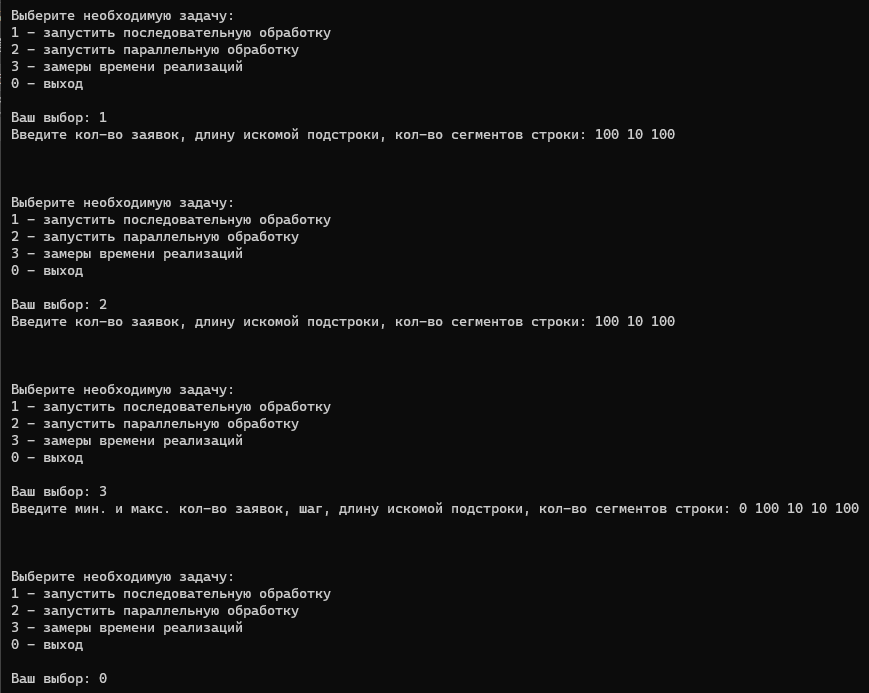
\includegraphics[width=0.4\linewidth]{images/example}
	\caption{Пример работы программы}
	\label{fig:example}
\end{figure}

\newpage

\subsection{Время выполнения реализованных алгоритмов}
Замеры времени работы реализованных алгоритмов для определенного размера квадратных матриц проводились 1000 раз, при этом каждый раз значения матриц генерировались случайно.

Для измерения тактового времени была использована инструкция rdtsc \cite{microsoft_rdtsc}.

В качестве результата, представленного на графике \ref{fig:timefull}, взято среднее время выполнения алгоритмов в тактах процессора для каждой матрицы размера от 1 до 10.

\begin{figure}
	\centering
	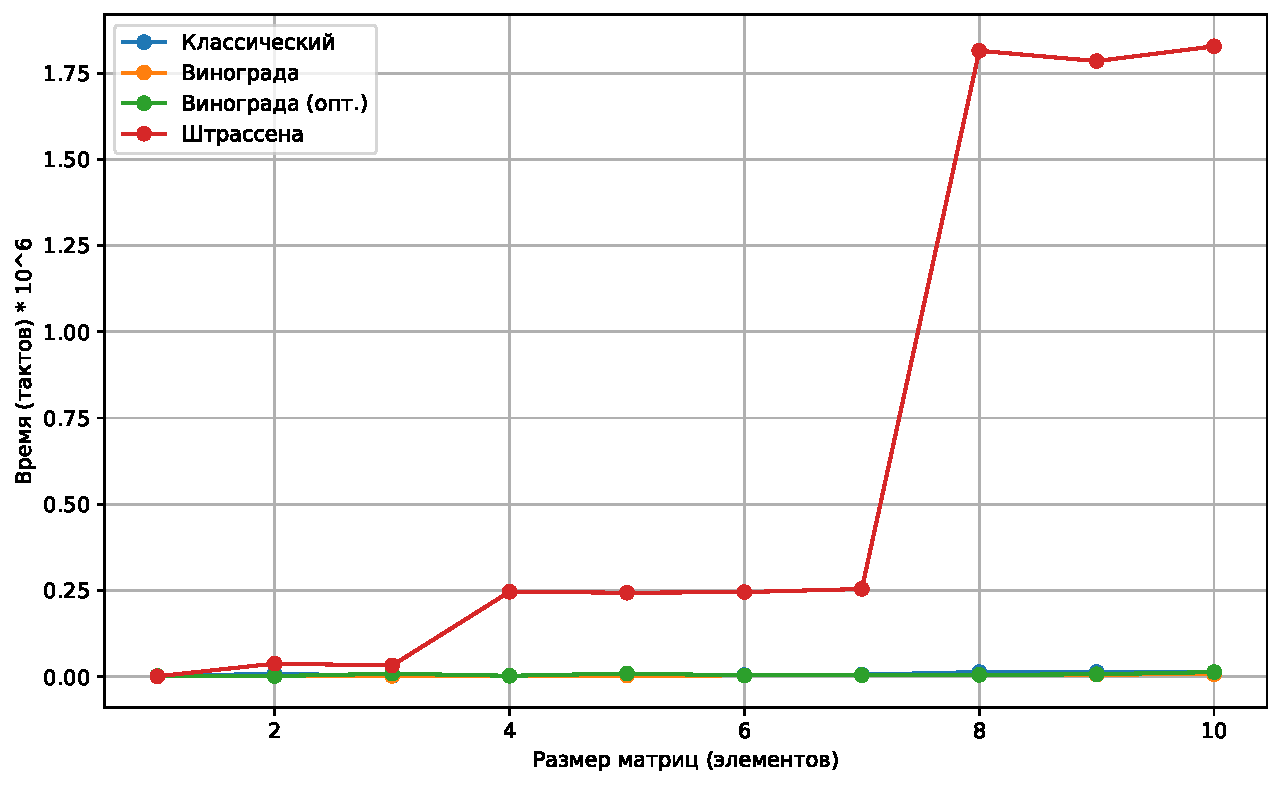
\includegraphics[width=0.9\linewidth]{../src/lab_02/timefull}
	\caption{Время выполнения алгоритмов}
	\label{fig:timefull}
\end{figure}

Тот же самый график, но без учёта алгоритма Штрассена:

\begin{figure}
	\centering
	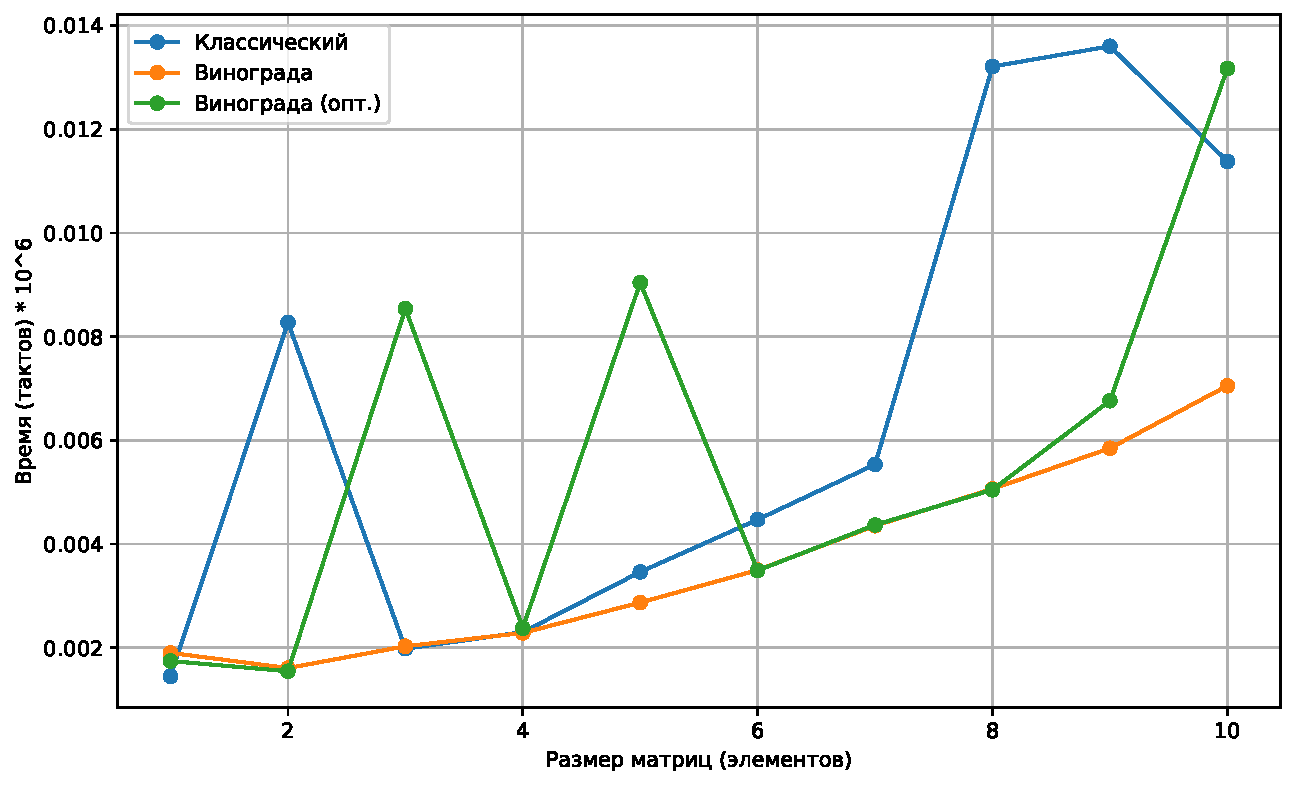
\includegraphics[width=0.9\linewidth]{../src/lab_02/time}
	\caption{Время выполнения алгоритмов (без учёта алгоритма Штрассена)}
	\label{fig:time}
\end{figure}

В половине случаев оптимизированная версия алгоритма Винограда работает дольше, чем \textit{обычный} алгоритм Винограда.

В результате трансляции кода программы на язык ассемблера, было замечено следующее: дизассемблированная строка исходного кода, выполняющая операцию вычисления значения \code{row[i]}, при оптимизированной реализации алгоритма Винограда содержит инструкции \code{lea} и \code{movsxd}, из-за чего количество выполняемых команд становится больше, чем в \textit{обычном} алгоритме Винограда.

Количество команд и, следовательно, разность в количестве инструкций также увеличивается при нечётном размере матриц.
Поэтому на графике заметны выбросы во времени у оптимизированного алгоритма Винограда.

Поэтому время выполнения увеличивается.

\newpage

\subsection{Занимаемая память реализованных алгоритмов}
 
График \ref{fig:memory} демонстрирует объём памяти в байтах, потребляемый разными реализациями алгоритмов в зависимости от размера матриц.
Занимаемый объём памяти считался как сумма размеров переменных, используемых в алгоритме и структуре данных.

\begin{figure}
	\centering
	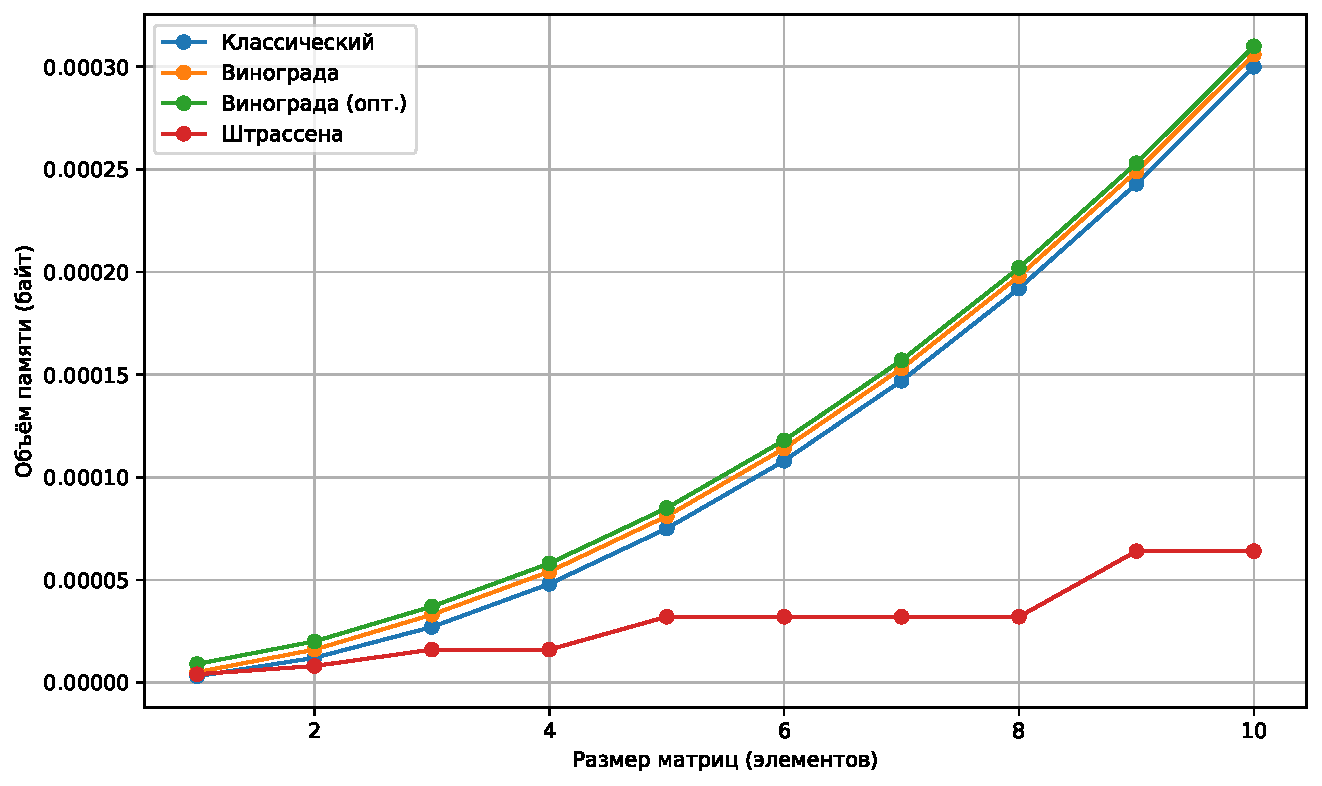
\includegraphics[width=0.9\linewidth]{../src/lab_02/memory}
	\caption{Объём памяти, используемый алгоритмами}
	\label{fig:memory}
\end{figure}


\subsection{Вывод}

В результате анализа замеров времени выполнения и затрат памяти на различных алгоритмах были сделаны следующие выводы:

\begin{itemize}
	\item алгоритм Штрассена занимает меньше всего памяти при размере квадратных матриц больше единицы;
	\item алгоритм Винограда и его оптимизированная версия быстрее всех умножают матрицы;
	\item разница во времени выполнения алгоритма Винограда и его оптимизированной версии зависит от процессора.
\end{itemize}
	\section*{ЗАКЛЮЧЕНИЕ}
\addcontentsline{toc}{section}{ЗАКЛЮЧЕНИЕ}

Цель работы достигнута, следующие задачи выполнены:
\begin{itemize}
	\item описана схема последовательного алгоритма поиска подстроки в строке методом полного перебора;
	\item разработано многопоточная версия данного алгоритма;
	\item описана схема алгоритма работы главного потока, который создаёт и запускает вспомогательные потоки;
	\item описана схема алгоритма вспомогательного потока;
	\item обоснована необходимость использования мьютексов и/или семафоров как примитивов синхронизации.
\end{itemize}


	\printbibliography
	
\end{document}
